\section{The Innovator's Method}

The Innovator's Method beschreibt eine Zusammenführung von etablierten Prozessen, um Schritt für Schritt ein erfolgreiches Startup aufzubauen.
Im Detail werden die Prozesse Sprint, The Lean Startup, sowie die Erstellung einer \ac{BMC} im Rahmen dieser Arbeit erklärt und umgesetzt.

\begin{figure}[h!]
	\begin{center}
		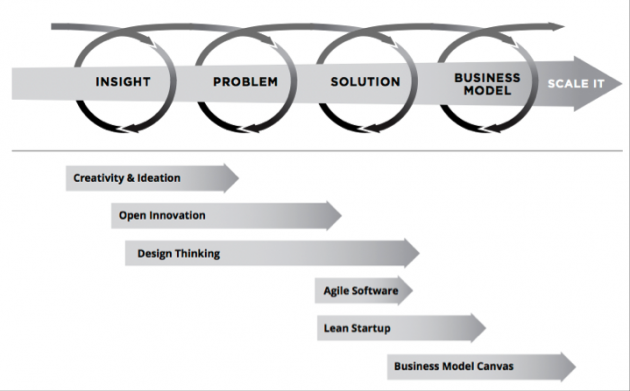
\includegraphics[width=\textwidth]{99_IMG/02_Grundlagen/innovatorsMethod.png}
		\caption{The Innovator's Method - Grundkonzept}
		\label{fig:TheInnovatorsMethod}
	\end{center}
\end{figure}

Allgemeiner gefasst, kann man The Innovator's Method in vier große Schritte aufteilen, wie in Abb. \ref{fig:TheInnovatorsMethod} dargestellt. Diese werden im Folgenden zusammengefasst erläutert.

\begin{enumerate}
	\item \textbf{Insight}
	
	In Schritt 1 liegt der Fokus darauf, die Zielgruppe zu beobachten, zu befragen und kennenzulernen. Erst wenn die Abläufe, welche die potentiellen Kunden zu durchlaufen haben, bekannt sind, kann daran angeknüpft werden. Nicht selten kommt es vor, dass überraschende Details erkannt werden, welche so ursprünglich nicht erwartet wurden. Das sind wesentliche Informationen, die ein kundenorientiertes Konzept ausmachen. Denn nur wenn alle Details über die kritische Ablauffolge klar sind, können daraus resultierende Probleme erkannt werden, wie im nächsten Punkt näher erklärt wird. 
	
	\item \textbf{Problem}
	
	Ein Problem kann hier auch ein Bedürfnis oder einen Wunsch erfüllen. Denn nicht immer löst ein neues Produkt ein bekanntes Problem. Meist werden daher Bedürfnisse erfüllt, von welchen der Nutzer ursprünglich nicht wusste, dass er sie hat. Um das herauszufinden, ist es essentiell, Schritt 1 so detailliert durchzuführen, dass diese Wünsche zum Vorschein kommen, ohne dass der Kunde sie formulieren muss. Das Problem per se muss dann gründlich herausgearbeitet werden, indem sich der Gründer in die Lage der Zielgruppe versetzt. Nur so ist es möglich, die entscheidenden Details, welche nicht auf den ersten Blick sichtbar sind, herauszufinden.
	
	\item \textbf{Solution}
	
	Die Lösung des vorher erarbeitetem und untersuchtem Problems soll nun prototypisiert werden. Im Vergleich zu einem fertig entwickelten Endprodukt hat ein Prototyp viele Vorteile. So kann eine Fassade des Produktes mit minimalem Entwicklungsaufwand ähnliches Feedback erzeugen. Obwohl das Problem bereits eingehend untersucht wurde, muss die entwickelte Lösung nicht zwingend optimal sein. Das heißt, das Problem ist bekannt, allerdings muss das optimale Konzept erst erarbeitet werden. Dazu ist es ineffizient, ein komplettes Produkt zu entwickeln, denn zuerst muss das Grundkonzept des Produktes getestet werden, nicht die Details. Dafür ist es ohnehin besser, dem Endnutzer einen Prototypen zur Verfügung zu stellen, damit dieser sich nicht an Einzelheiten aufhängt. Außerdem ist der emotionale Wert des Produktes höher, wenn in dieses bereits viel Zeit investiert wurde. Nachdem das Konzept unter Umständen im Test durchfällt und dann neu entwickelt werden muss, soll dies vermieden werden. Zusammenfassend sollen also grobe Prototypen von den Endnutzern validiert werden, um die optimale Lösungsstrategie herauszufinden und auf den Kunden abzustimmen - welcher letztendlich den Markterfolg bestimmt.
	
	\item \textbf{Business Model}
	
	Erst nachdem bekannt ist, was der Endkunde braucht und wie dieser Wunsch erfüllt werden kann, wird die Marktstrategie erarbeitet. Das gesamte Wissen über die Zielgruppe ist hier erneut sehr wichtig. Denn ein Produkt, welches zwar optimal auf den Kunden abgestimmt ist, ist nicht wertbringend, wenn die Zielgruppe nicht weiß, dass dieses Produkt exisitert. Daher muss der ideale Weg gefunden werden, die Ware an den Kunden zu bringen. 
\end{enumerate}

Für jeden dieser Schritte sind unter Umständen mehrere Anläufe nötig. Selten schafft es ein Team, die idealen Ergebnisse in einer Iteration zu bekommen. Doch auch fehlgeschlagene Anläufe sind wertvoll, da das Team aus Irrtümern wiederum wichtige Einblicke in die Kundensicht erlangt. 
\cite{TheInnovatorsMethod}
\newpage 